\documentclass[aps,nofootinbib,prl,twocolumn,superscriptaddress]{revtex4}

\usepackage[strict]{revquantum}


%% PATHS %%

\newcommand{\figurefolder}{../fig}


%% OTHER NOTATION %%

% Normalize spelling, font decoration.
\newcommand{\mps}{x}
\newcommand{\eps}{e}
\newcommand{\data}{d}

\newcommand{\MLE}{\text{MLE}}
\newcommand{\ESM}{\text{ESM}}

\renewcommand{\H}{H}
\newcommand{\uw}{{\mu\text{w}}}


% http://tex.stackexchange.com/a/112947/615
\newcommand{\apxref}[1]{\hyperref[#1]{Appendix~\ref{#1}}}

%=============================================================================
% FRONT MATTER
%=============================================================================

\begin{document}

\title{Adaptive Online Experiment Design with Quantum Systems}

\author{Ian Hincks}
\affilUWAMath
\affilIQC

\author{Thomas Alexander}
\affilUWPhys
\affilIQC

\author{Michal Kononenko}
\affilTODO

\author{Benjamin Soloway}
\affilTODO

\author{David G. Cory}
\affilUWChem
\affilIQC
\affilPI
\affilCIFAR

% new authors add your names

\date{\today}

\begin{abstract}
    Aliquam maximus sem ut imperdiet pulvinar. Donec ut sagittis metus, vitae congue risus. Vestibulum ut mi pharetra, commodo risus eget, consequat sapien. Integer vulputate dolor nec nisl sodales, quis condimentum nulla mollis. Curabitur molestie lacus eget accumsan elementum. 
\end{abstract}

\maketitle

%=============================================================================
% MAIN DOCUMENT
%=============================================================================



%=============================================================================
\section{Introduction}
\label{sec:intro}
%=============================================================================

 Lorem ipsum dolor sit amet, consectetur adipiscing elit. Pellentesque quis tellus in lorem fermentum vehicula. Cras placerat ante arcu, vitae porta felis sodales ac. Orci varius natoque penatibus et magnis dis parturient montes, nascetur ridiculus mus. Fusce turpis velit, mattis vel lectus nec, aliquam molestie ligula. Nam sollicitudin, urna cursus ultricies molestie, orci metus aliquet odio, vel consectetur augue tortor in neque. Donec posuere diam nec ligula laoreet fringilla. Proin diam dui, hendrerit eu tortor vel, ultrices maximus mi. Phasellus sodales finibus massa nec porttitor. Ut posuere tortor id ante lobortis iaculis at at ex. Phasellus in ligula suscipit, pulvinar est at, mollis est. Fusce rutrum pretium lacus commodo ultricies. In porttitor mi mauris, sollicitudin facilisis neque scelerisque at.

%=============================================================================
\section{Inference of Quantum Devices}
\label{sec:inference}
%=============================================================================

We begin by defining some notation while reviewing parameter 
estimation as applied to quantum devices.

Information about a quantum device can be encoded into a list of 
real values, which we call \textit{model parameters}, labeled $\mps$.
For example, in the case of Hamiltonian learning, 
these values parameterize the Hamiltonian operator of the 
quantum system, or in the case of 
state tomography, the entries of a density operator.
This set of parameters includes both parameters of interest, which 
one is interested in learning, and nuisance parameters, which are
not of principle interest, but are still necessary to sufficiently 
describe the system.

Quantum devices are controlled by some collection of 
classical knobs that adjust various settings 
such as power levels, timings, input frequencies, and so on.
We refer to a specific assignment of all of these settings as an
\textit{experiment configuration}, which we label $\eps$.
Then an \textit{experiment}
consists of a quantum measurement (or set of quantum measurements) 
made using these fixed experiment configuration.
For example, in this nomenclature, a standard Rabi curve 
would be constructed by making a set of 
experiments, each one defining---among other fixed parameters---a 
pulsing time in its experimental configuration, 
$\eps=(\ldots,t_\text{pulse},\ldots)$.

An experiment returns a datum $\data$. 
This might be a photon count
over a known time interval, a time series of voltages, 
or a number of `down' strong measurement results out of $N$ repetitions
of the configuration, and so on.

Generally, the goal of statistical inference is to learn about the parameters
$\mps$ given a data set $\data_1,\ldots,\data_n$ with respective 
configurations $\eps_1,\ldots,\eps_n$.
This requires us to additionally specify a model for the 
system---something which connects the model parameters to the experiment 
configurations and data.
This is done through a likelihood function,
\begin{equation}
    \Lhood(\mps;(\data_1,\eps_n),\ldots,(\data_n,\eps_n))
        = \Pr(\data_1,...,\data_n|\mps,\eps_1,...,\eps_n),
\end{equation} 
which returns the probability of receiving a given dataset conditioned
on a hypothetical configuration $\mps$.
Note that multiple models can be considered and compared if the
true model is not known, if such a thing even exists.
For quantum systems, these likelihood models come naturally
through quantum system evolution formulas in conjunction 
with Born's rule.

One popular inference choice is to maximize the likelihood function
with respect to $\mps$, producing the maximum likelihood estimate (MLE) 
$\hat{\mps}_\MLE:=\operatorname{argmax}_\mps \Lhood$.
Confidence regions of this estimate can be constructed 
with statistical derivations, or more generally, through techniques like bootstrapping.
Least-squared curve fitting is often used as a proxy for the MLE (with 
confidence intervals arriving from assuming
a linearized model) since it is exactly equal to the MLE
for linear models.

The MLE is one example of an estimator in a vast literature on estimator theory.
In this Letter, we limit ourselves to the use of Bayesian inference because of its
natural integration with online experiments, discussed below.
In short, in the paradigm of Bayesian inference, one constantly
maintains a state of knowledge about the model parameters $\mps$, encoded
as a probability distribution $\Pr(\mps)$.
Upon receiving any piece of data $\data$ under configuration $\eps$,
our state of knowledge is updated from $\Pr(\mps)$ to $\Pr(\mps|\data,\eps)$
through Bayes' law:
\begin{equation}
    \Pr(\mps|\data,\eps)
        = \frac{\Pr(\data|\mps,\eps)\Pr(\mps)}{\Pr(d)}.
\end{equation}
In most numerical implementations of this law, the denominator of the 
right and side comes out in the wash, and we are left with
\begin{equation}
    \Pr(\mps|\data,\eps)
        \propto \Lhood(\mps;\data,\eps)\Pr(\mps),
\end{equation}
the product of our prior state of knowledge and the likelihood
of the hypothetical model parameter value $\mps$.

%=============================================================================
\section{Experiment Design}
\label{sec:experiment-design}
%=============================================================================

An \textit{experiment design heuristic} is simply a function that 
determines the next experiment configuration to use.
We say such a heuristic is \textit{online} if it explicitly uses the current
state of knowledge to make its choice, and we call it \textit{offline} 
otherwise.
Conventionally, as an example, Rabi curves are generated 
with offline heuristics, where the next experiment is chosen by 
increasing the pulse time by a fixed duration in each experiment.
The number of experiments and pulse time increments are chosen through
Nyquist considerations.

%=============================================================================
\section{System Model}
\label{sec:system-model}
%=============================================================================

The quantum system used in our experiment is a nitrogen vacancy (NV) center,
which is a defect in diamond consisting of a nitrogen adjacent to 
a vacant lattice position.
When in its stable negatively charged configuration, NV$^-$, 
the vacancy is filled with
six electrons that form an effective spin-1 particle in the optical
ground state---this three level subspace comprises the system of interest.
The eigenstates are labeled $\ket{0}$, $\ket{-1}$, and $\ket{+1}$.
There is a zero field splitting (ZFS) of $D\approx\SI{2.87}{GHz}$ 
between $\ket{0}$ and the $\ket{-1},\ket{+1}$ manifold 
that---at low fields ($\lesssim\SI{100}{G}$)---is the dominant energy term,
defining our $z$-axis.
The Zeeman splitting between $\ket{-1}$ and $\ket{+1}$ is determined by
the magnetic field projection onto the $z$-axis, equal to
$\omega_e=\gamma_e |B_z|$ in the secular approximation, 
where $\gamma_e=\SI{2.80}{MHz/G}$.
Spin manipulation is achieved with resonant microwave driving near
the transitions $D\pm\omega_e$.
Long coherence times are observed at room temperature, where
the spin state can be initialized and measured optically, and single 
defects are studied in isolation using confocal microscopy.

In the rotating frame, with the rotating wave and secular approximations,
the Hamiltonian of the optical ground state is given by
\begin{align}
    \H/2\pi &= (D-\omega_\uw)\Sz^2 + (\omega_e+A \Iz)\Sz + \Omega(t)\Sx
\end{align}
where $(\Sx,\Sy,\Sz)$ are the spin-1 operators, $\omega_\uw$ is the applied
microwave frequency, $\Omega(t)$ is the microwave drive strength, $A$ is
the hyperfine splitting  due to the adjacent nitrogen-14 atom, and $\Iz$
is the nitrogen spin-1 operator along $z$.
Along with the $T_2^*$ decoherence time which introduces the 
Lindblad operator $L=\sqrt{1/T_2^*}\Sz$, these parameter are sufficient
to simulate the experiments we perform.
Therefore, the model parameters of our spin system are given by
\begin{align}
    \mps=(\Omega,\omega_e,A,
\end{align}



%=============================================================================
\section{Implementation}
\label{sec:implementation}
%=============================================================================

We implement  \autoref{tab:heuristics}.

\begin{table*}[t]
    \centering
    \begin{tabularx}{\textwidth}{lX}
        \textbf{Heuristic} & \textbf{Definition} \\
        \hline \\
        Alternating Linear &  \\
        Online Risk
    \end{tabularx}
    \caption{Summary of heuristics used in experiments.}
    \label{tab:heuristics}
\end{table*}    

%=============================================================================
\section{Results}
\label{sec:results}
%=============================================================================

\begin{figure*}
    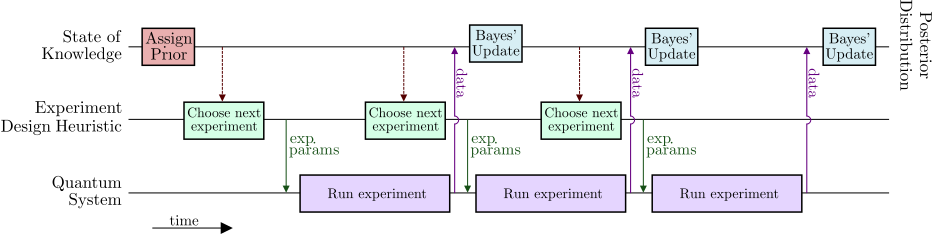
\includegraphics[width=\textwidth]{\figurefolder/online-timing-diagram}
    \caption{Timing diagram for three rounds of online learning. The role of the
    experiment design heuristic is to pick the next experiment, possibly based
    on the current state of knowledge (i.e. probability distribution over parameters
    of interest). This choice might be computationally expensive, and is 
    therefore run concurrently with quantum experiments.}
    \label{fig:online-timing-diagram}
\end{figure*}

%=============================================================================
\section{Conclusions}
\label{sec:conclusions}
%=============================================================================

Nulla commodo felis a est tincidunt porttitor. Praesent venenatis tellus eget ipsum tempus, sit amet tempus dui venenatis. Sed vel massa fermentum, cursus tellus ultricies, lacinia turpis. Donec rhoncus finibus semper. Pellentesque leo nunc, vehicula id tempor sit amet, tempus non nisi. Aliquam non faucibus nisi, quis dapibus odio. Duis ullamcorper nunc ultricies suscipit aliquam. Phasellus quis molestie eros, nec convallis justo. Integer massa diam, interdum quis diam ut, elementum luctus quam. Nullam interdum orci nec ultricies scelerisque. Praesent eget commodo tortor. In et risus vitae felis mollis hendrerit ut ac lacus. Maecenas congue sollicitudin erat, a eleifend nulla euismod ullamcorper. Nullam accumsan sodales metus. Vestibulum ante ipsum primis in faucibus orci luctus et ultrices posuere cubilia Curae; Pellentesque feugiat quam at justo tincidunt euismod. 

%=============================================================================
% END MATTER
%=============================================================================

\acknowledgments{
    
}

\bibliographystyle{apsrev4-1}
\bibliography{nv-adaptive}

%=============================================================================
% APPENDICES
%=============================================================================

\appendix
\onecolumngrid

%=============================================================================
\section{Effective Strong Measurements}
\label{apx:effective-strong-measurements}
%=============================================================================

Given a quantum state $\rho$, 
information is accessed through the
Born's probability $p=\Tr(\ketbra{0}\rho)$.
In the hypothetical case of strong measurement, in the language
of statistics, we would be able to draw from 
the Bernoulli distribution $\bernoullidist(p)$, or more generally, with 
$n$ repeated preparations and strong measurements, from 
the binomial distribution $\binomialdist(n,p)$.

Standard room temperature NV setups do not allow strong measurements. 
Instead, access to the quantity $p$ is obstructed by three Poisson rates,
such that conditional on some values $0<\beta<\alpha$, we can 
draw from the random variables
\begin{align}
    X|\alpha &\sim \poissondist(\alpha) \nonumber \\
    Y|\beta &\sim \poissondist(\beta) \nonumber \\
    Z|\alpha,\beta,p &\sim \poissondist(p\alpha + (1-p)\beta).
\end{align}
The quantities $\alpha$ and $\beta$ are known as the bright reference
and the dark reference, respectively.
They are defined as the 
expected number of photons collected (and summed over $N$
repetitions of the experiment) using the initial NV states
$\ketbra{0}$ and $\ketbra{1}$, respectively\footnote{They are
more accurately defined in terms of the pseudo-pure states 
that are actually created in the NV initialization procedure~\cite{hincks_statistical_2017}.}.

The information content about $p$ of this referenced Poisson model is not
immediately obvious, 
and depends both on the magnitude of $\alpha+\beta$, 
as well as the contrast between $\alpha$ and $\beta$.
This is different than the strong measurement case mentioned above,
where $n$ strong measurements has a clear intuitive and operational 
interpretation.
The goal of this section is to reduce information about the references
$\alpha$ and $\beta$ into a single number 
with the same interpretation as $n$.
This will allow one, for example,
to quantitatively compare two experimental setups or NVs and
decide which one is better at providing information about $p$. 

It has been shown\cite{hincks_statistical_2017} that the 
Fisher information matrix of this 
referenced Poisson model is given by
\begin{align}
    J(p,\alpha,\beta) &=
        \begin{pmatrix}
            \frac{(\alpha -\beta )^2}{p (\alpha -\beta )+\beta } & 
            \frac{p (\alpha -\beta )}{p (\alpha -\beta )+\beta } & 
            \frac{\alpha }{\beta +\alpha  p-\beta  p}-1 \\
            \frac{p (\alpha -\beta )}{p (\alpha -\beta )+\beta } & 
            \frac{p^2}{p \alpha -p \beta +\beta }+\frac{1}{\alpha } & 
            -\frac{(p-1) p}{p (\alpha -\beta )+\beta } \\
            \frac{\alpha }{p \alpha -p \beta +\beta }-1 & 
            -\frac{(p-1) p}{p (\alpha -\beta )+\beta } & 
            \frac{p \alpha +(p-2) (p-1) \beta }{\beta  (p (\alpha -\beta )+\beta )} \\
        \end{pmatrix}
\end{align}
with inverse matrix
\begin{align}
    J(p,\alpha,\beta)^{-1}
        &=
        \begin{pmatrix}
            \frac{p (p+1) \alpha +(p-2) (p-1) \beta }{(\alpha -\beta )^2} & 
            \frac{p \alpha }{\beta -\alpha } & 
            \frac{(p-1) \beta }{\alpha -\beta } \\
            \frac{p \alpha }{\beta -\alpha } & 
            \alpha  & 
            0 \\
            \frac{(p-1) \beta }{\alpha -\beta } & 
            0 & 
            \beta
        \end{pmatrix}.
\end{align}

Using the Cramer-Rao bound, these matrices let us
estimate the information content of $p$ in the referenced
Poisson model.
Specifically, they give us an estimate in each of the following 
extreme cases.
First, the $(p,p)$ element of $J^{-1}$, 
$(J^{-1})_{p,p}=\frac{p (p+1) \alpha +(p-2) (p-1) \beta }{(\alpha -\beta )^2}$,
is a lower bound on the variance of any (unbiased) estimate of $p$ given that
a single measurement of the triple $(X,Y,Z)$ has been made, 
with no prior information
about $p$, $\alpha$, or $\beta$ given.
Second, the inverse of the $(p,p)$ element of $J$,
$(J_{p,p})^{-1}=\frac{p (\alpha -\beta )+\beta}{(\alpha -\beta )^2 }$,
 is a lower bound on 
the variance of any (unbiased) estimate of $p$ given that a single 
measurement of $Z$ has been made, assuming perfect knowledge of
both $\alpha$ and $\beta$.

It will be useful for us to also be able to interpolate between these two
extremes, where some, but not all, prior information 
about $\alpha$ and $\beta$ is available.
There are a few tacks that one might consider to achieve this, including
the Bayesian Cramer-Rao bound, or looking directly at the risk of some 
estimator.
Instead, we choose a slightly ad-hoc method as it actually produces 
a tractable calculation---statistics of the referenced Poisson model
usually involve a triple infinite sum, and many calculations are simply
not possible without numerics.
To this end, let $\sigma_\alpha^2$ and $\sigma_\beta^2$ represent 
our prior variances of $\alpha$ and $\beta$, respectively, before
taking a measurement of $Z|\alpha,\beta,p$.
We can now ask the question: how many times, $M$, we must measure 
$X|\alpha$ and $Y|\beta$ to produce these variances in the first 
place?
We must allow $M$ to depend on $\alpha$ or $\beta$ in each case.
The distribution $\poissondist(M(\lambda)\lambda)$ has 
Fisher information given by 
$\frac{(M(\lambda)+\lambda M'(\lambda))^2}{\lambda M(\lambda}$.
Equating this to $1/\sigma^2$ and soliving the differential
equation at $M(0)=0$ gives $M=\lambda/4\sigma^2$.
Therefore consider the distribution
\begin{align}
    \poissondist\left(\frac{\alpha^2}{4\sigma_\alpha^2}\right)
        \times \poissondist\left(\frac{\beta^2}{4\sigma_\beta^2}\right)
        \times \poissondist\left(p\alpha+(1-p)\beta\right)
\end{align}
which effectively results in our desired information about $\alpha$
and $\beta$.
Solving for the $(p,p)$ element of the inverse Fisher information
matrix of this distribution results in the formula
\begin{align}
    K=\frac{
        \beta +p\left(\alpha-\beta+p \sigma_\alpha ^2
        +(p-2) \sigma_\beta ^2\right)+\sigma_\beta ^2}{(\alpha -\beta )^2}.
\end{align}
This formula correctly interpolates between the case of perfect prior 
information, and prior information as collected by a single sample
of $(X,Y)|\alpha,\beta$, namely,
\begin{align}
    \lim_{\sigma_\alpha^2,\sigma_\beta^2\rightarrow 0} K 
        &= (J_{p,p})^{-1} \quad\quad\text{and}\quad\quad
    \lim_{\sigma_\alpha^2\rightarrow \alpha, \sigma_\beta^2\rightarrow \beta} K 
        = (J^{-1})_{p,p}.
\end{align}

The inverse Fisher information of the binomial model $\binomialdist(n,p)$
is given by $\frac{p(1-p)}{n}$, which when integrated uniformly over 
$[0,1]$, produces $\frac{1}{6n}$.
Our definition for the number of effective strong measurements (ESM)
of a referenced Poisson model with parameters 
$(\alpha,\beta,\sigma_\alpha,\sigma_\beta)$ is defined by 
equating $\int_0^1 K\dd p=\frac{1}{6n}$ and solving for $n$,
which results in
\begin{align}
    n_\ESM = \frac{
            (\alpha-\beta)^2
        }{
            3(\alpha+\beta)+2\left(\sigma_\alpha^2+\sigma_\beta^2\right)
        }.
\end{align}
This shows, for example, 
that having perfect information about $\alpha$ and $\beta$
before measuring $Z|\alpha,\beta,p$ is roughly equivalent---in terms
of information learned about p---to 
$5/3\approx 1.67$ times more effective strong measurements 
than the case where the triple $(X,Y,Z)|\alpha,\beta,p$ is
measured, but with no prior information.

Finally, in \autoref{fig:effective-strong-meas}, we use some numerics
to show that the $\ESM$
quantity accurately relates the mean-squared error of the Bayes estimator
for the referenced Poisson model and a binomial model with $n=n_\ESM$.

\begin{figure}
    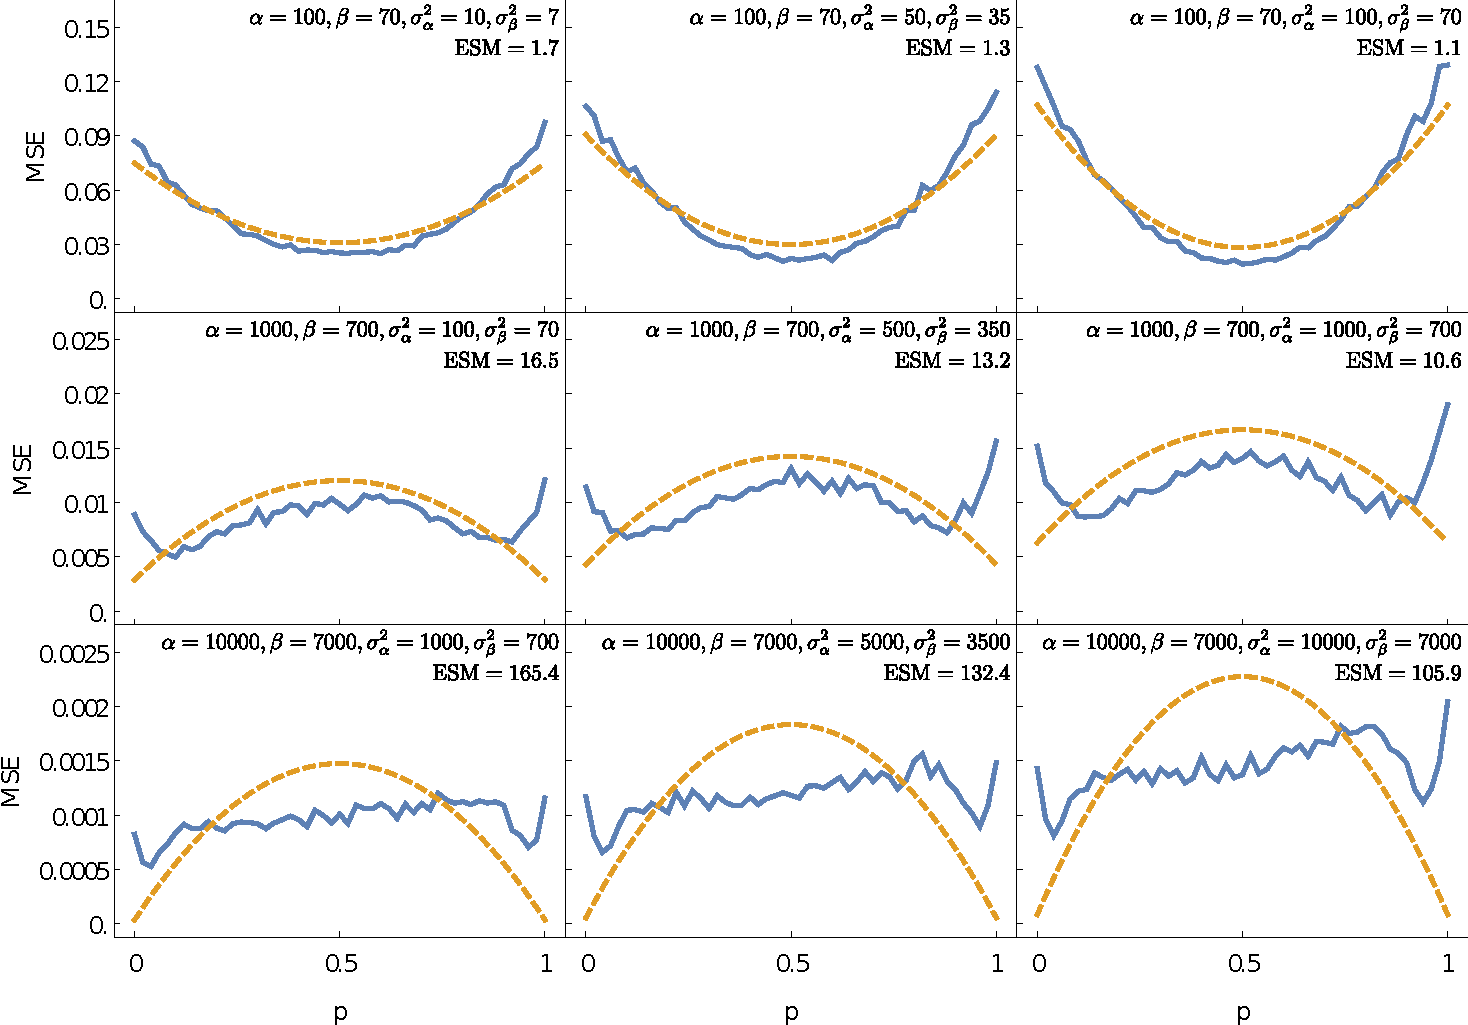
\includegraphics[width=\textwidth]{\figurefolder/effective-strong-meas}
    \caption{The mean-squared-error of the Bayes estimator is computed
    as a function of $p$
    for both the referenced Poisson model (blue, solid) and for a binomial model
    (orange, dashed) where $n=n_\ESM$.
    The prior distribution on $p$ is uniform.
    This is done in nine regimes, corresponding to the nine subplots of the figure.
    Each row uses a different magnitude of bright reference, $\alpha$,
    and each column uses a different amount of prior reference knowledge.
    The left column uses sub-Poisson error bars on $\alpha$ and $\beta$,
    and the right column uses regular Poisson error bars.}
    \label{fig:effective-strong-meas}
\end{figure}

%=============================================================================
\section{Simulation the Nitrogen}
\label{apx:nitrogen-sim}
%=============================================================================

The nitrogen atom adjacent to the vacancy couples to our system with
an isotropic hyperfine interaction, $A\cdot\Sz\otimes\Iz$.
Therefore, for a given experiment, we treat it as a small fixed magnet
with strength $m_I A$, where $m_I\in\{-1,0,+1\}$ is its current eigenstate,

This is justified due to its long $T_1$ time with respect to a single
experiment---in 

%=============================================================================
\section{Risk Approximations}
\label{apx:risk-approximations}
%=============================================================================

%=============================================================================
\section{BCRB for Hamiltonian Learning}
\label{apx:bcrb}
%=============================================================================



\end{document}
